\chapter{Case Study: UAS operating in the NAS} \label{ch:UASinNAS}

According to the integration of civil Unmanned Aerial Systems into the Nation Airspace System roadmap~\cite{nasroadmap} the FAA is working with other government agencies and industry to develop a collaborative UAS modeling and simulation environment to explore key challenges to UAS integration. The near-term modeling goals are to:
\begin{itemize}
  \item Validate current mitigation proposals
  \item Establish a baseline of end-to-end Unmanned Aerial System performance measures
  \item Establish thresholds for safe and efficient introduction of Unmanned Aerial Systems into the National Airspace System
  \item Develop NextGen concepts, including 4-dimensional trajectory utilizing Unmanned Aerial Systems technology
\end{itemize}

We believe that the Model Abstraction Framework accomplishes each of these goals.  The framework is extremely flexible, allowing it to model a large variety of systems at varying and alternating degrees of abstraction, an attribute that is ideal for new designs.  It has the ability to detect critical failures.  It has the ability to examine multiple paths through the model and to randomly perturb the model in different ways to explore these paths.  It also generates human workload metrics that are valuable for setting safety thresholds and analyzing new designs.

The roadmap~\cite{nasroadmap} also identifies several interrelated research challenges:
\begin{itemize}
  \item Effective human-automation interaction (level of autonomy; trust; and mode awareness)
  \item Pilot-centric ground control station design (displays; sensory deficit and remediation; and sterile cockpit)
  \item Display of traffic/airspace information (separation assurance interface)
  \item Predictability and contingency management (lost link status; lost ATC communication; and ATC workload)
  \item Definition of roles and responsibilities (communication flow among crew, ATC, and flight dispatcher)
  \item System-level issues (NAS-wide human performance requirements)
  \item Airspace users� and providers� qualification and training (crew/ATC skill set, training, certification, and currency)
\end{itemize}

The Model Abstraction Framework was specifically designed to model human-automation interaction for UAS.  Our WiSAR model specifically demonstrates predictability and contingency management for each path in the model.  The DiRG allows us to model specific roles and their responsibilities while the DiTG defines communication flow between different roles.  And the workload metrics allow models of human performance to be verified.

Due to the nearly identical nature of the FAA's goals with our own, we have modeled a basic Unmanned Aerial System integrating into the National Airspace System.  Due to our lack of domain knowledge we have had to make a number of assumptions in order to achieve a high level of abstraction.  Despite the high level of abstraction we believe that the results are informative.

\section{Model Scenario and Assumptions}

  To help illustrate this model we have created a DiRG that shows the states and data flow for each Actor.  Figure~\ref{fig:uasnasdirg}.  A matching DiTG for the model showing the Actor communication channels can be seen in figure~\ref{fig:uasnasditg}.

An Unmanned Aerial System (UAS) plans to operate within the National Airspace System.  The UAS is composed of a server (UAS Server), an Unmanned Aerial Vehicle Operator (UAV Operator), and an Unmanned Aerial Vehicle (UAV).  The UAV Operator controls the UAS Server through a graphical user interface (UAS GUI) that in turn controls the UAV, as illustrated in the DiTG shown in figure~\ref{fig:uasnasditg}.  The UAV will take off and land at an airport serving both manned and unmanned aerial vehicles.  The UAV Operator is located at this airport and visually monitors the takeoff and landing of the UAV.  UAV state is continuously shown on the UAS GUI.

\begin{figure}[h]
\begin{center}
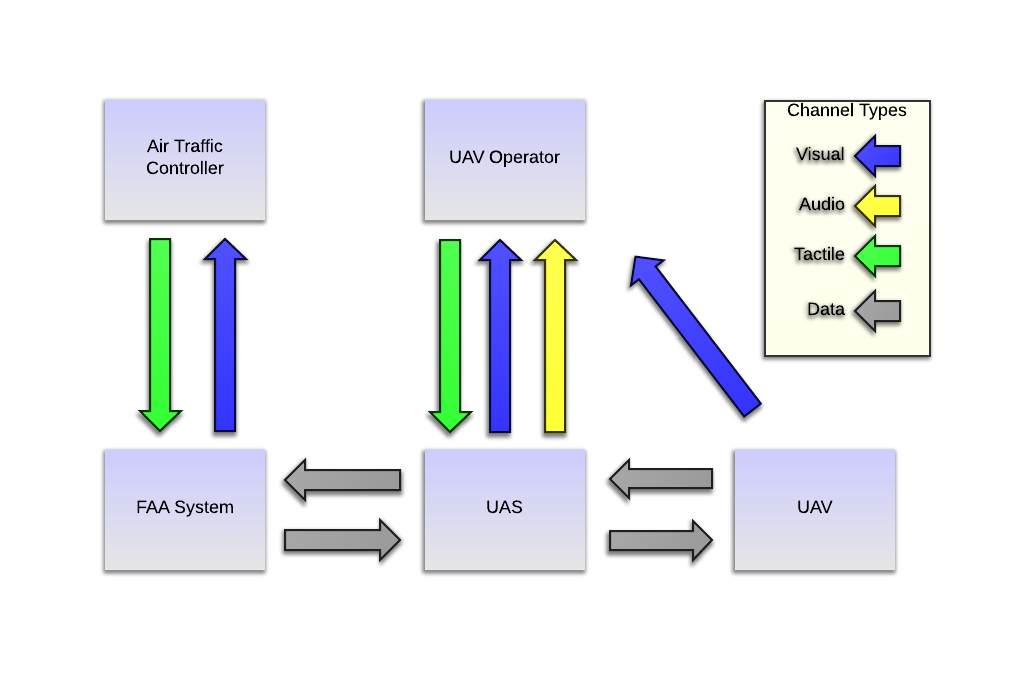
\includegraphics[width=5in]{uasnasditg.png}
\caption{DiTG: UAS integration into the NAS Model}
\label{fig:uasnasditg}
\end{center}
\end{figure}

There is an FAA Server that provides real-time notice to airmen (NOTAM) information.  The UAS Server connects to this server, receives the NOTAMs and displays them on the UAS GUI.  Figure~\ref{fig:uasnasditg}.  The FAA system also allows the UAS Server to file flight plans.  Filed flight plans are automatically checked for simple conflicts such as crossing NOTAMS or duplicate takeoff/landing times.  If there is a conflict the FAA Server flags the flight plan for an Air Traffic Controller (ATC) and displays these requests on an FAA GUI that is monitored by the ATC.  The ATC then approves or denies flight plans, using the FAA GUI, at their leisure.  This approval/denial then becomes available to the UAS Server, which displays it on the UAS GUI as illustrated in the DiRG shown in Figure~\ref{fig:uasnasdirg}.

\begin{figure}[h]
\begin{center}
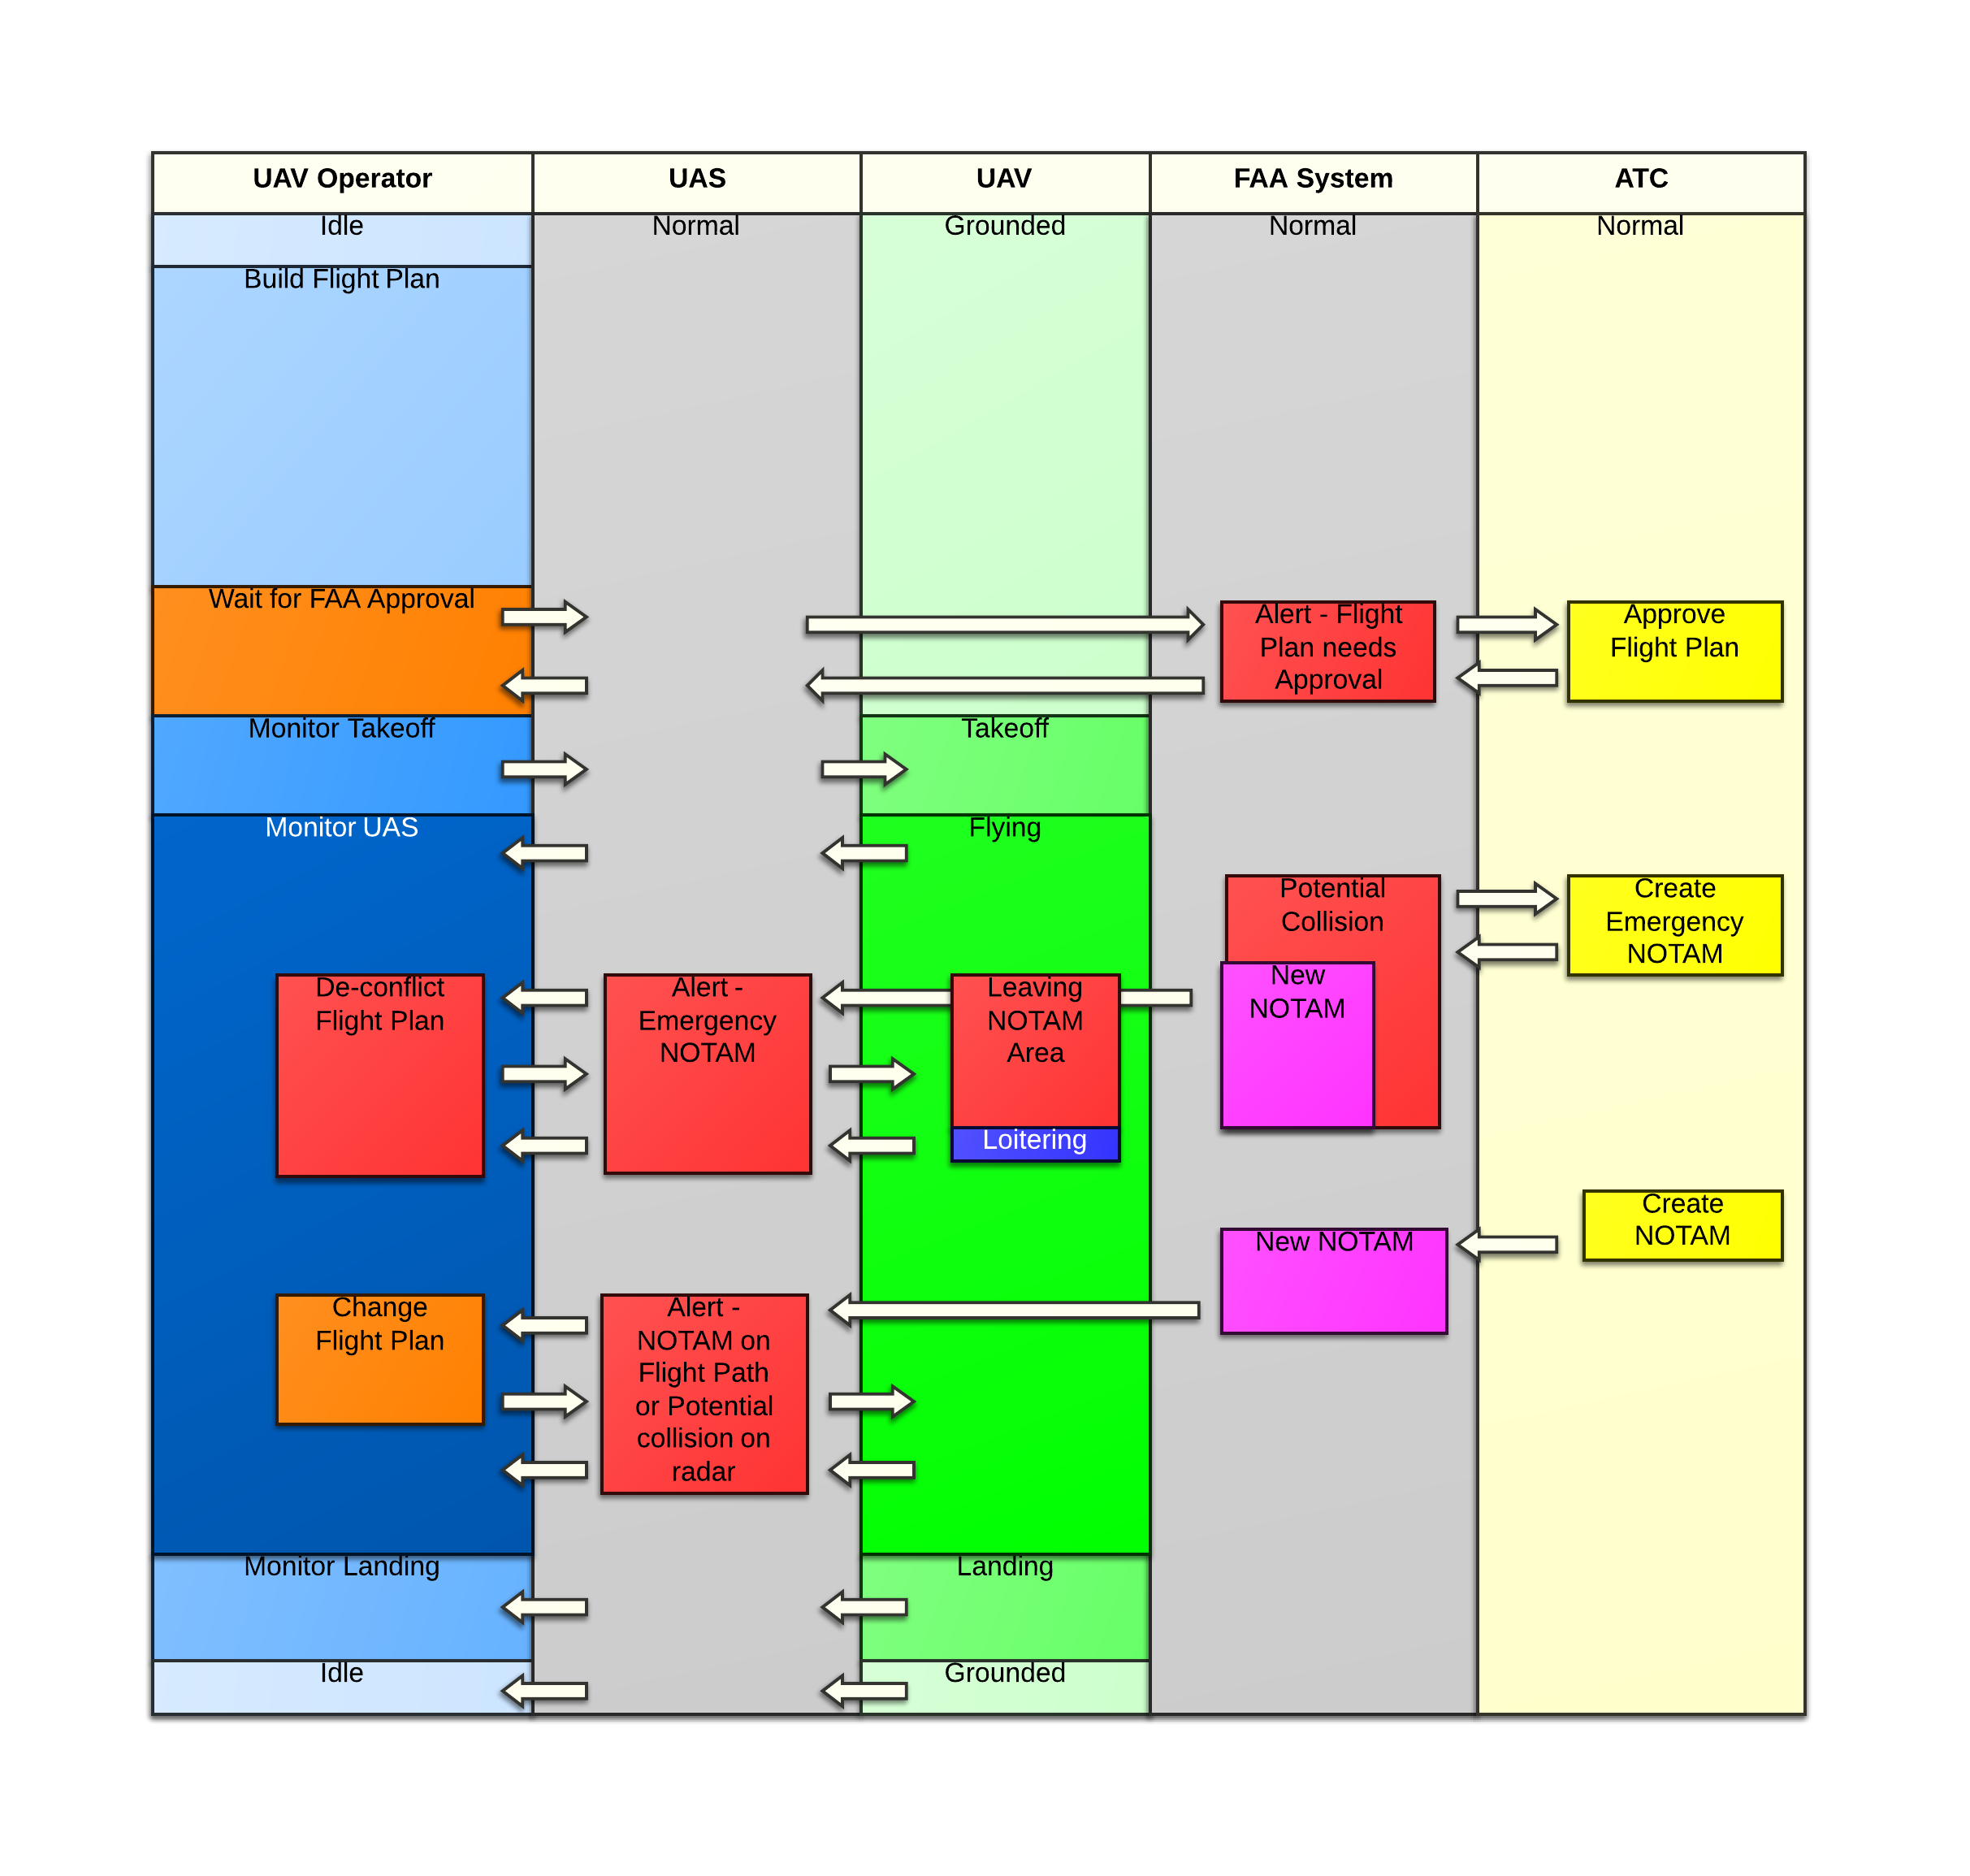
\includegraphics[width=6in]{uasnasdirg.png}
\caption{DiRG: UAS integration into the NAS Model.  Columns represent Actors, column sections represent states, and arrows represent inter Actor data flow.}
\label{fig:uasnasdirg}
\end{center}
\end{figure}

The FAA Server also provides radar information to the ATC through the FAA GUI.  The ATC uses this information to spot potential collisions with UAVs.  If a potential UAV collision is detected the ATC creates an emergency NOTAM in the region of conflict.  This emergency NOTAM is then sent to the UAS Server, which displays the emergency NOTAM on the UAS GUI.  If the UAV is in or near the emergency NOTAM it must change course to immediately evacuate/avoid the NOTAM.  This can be done automatically by the UAV or manually by the UAV Operator.  Once the UAV has finished avoiding the emergency NOTAM it enters a loiter state.  The UAV Operator is then required to change the flight plan before the UAV will leave the loiter state.  Figure~\ref{fig:uasnasdirg}.

The UAV also has a radar that can detect nearby objects.  This information is displayed on the UAS GUI and if the UAV Operator detects a potential collision they will begin the deconfliction procedure that requires changing the current flight plan.  Once the UAV has landed the scenario is considered complete.

\subsection{Assumptions}

The number of assumptions made in this scenario is too great to fully list.  Instead we have only attempted to list the major assumptions that are required for the model to perform as designed.
\begin{itemize}
  \item The UAV has an unlimited flight time, never loses contact with the UAS Server, can takeoff and land without incident, has accurate GPS data, and is non line-of-sight.
  \item The UAS Server/GUI never loses connection to the FAA Server, always has instant communication with the UAV and FAA Server, has no bugs, can create flight plans, can detect NOTAMs on the flight plan, can automatically direct the UAV out of an emergency NOTAM, displays radar information from the UAV, and never goes down.
  \item The UAV Operator detects all warnings displayed on the UAS GUI, generates flight plans that do not touch NOTAMS, can always deconflict the UAV, and never gets fatigued.
  \item The FAA Server/GUI distributes NOTAMS and automatically detects if a flight plan needs to be approved by the ATC.
  \item The ATC detects all information displayed on the FAA GUI, can add NOTAMS with the FAA GUI, always adds NOTAMS correctly, and approves all flight plans.
\end{itemize}

\section{Building the Model}

Initially working with a single XML file instead of multiple Java class files was very convenient.  Additionally the ability to validate the model each time we added a new transition led to very rapid development.  The simplified syntax also made construction easier.  Figure~\ref{fig:read_transition} shows two different transitions, one in Java and the other in XML.  Determining the inputs, outputs, end state, and more is much easier to do with the XML transition because of the hierarchical structure and the smaller syntax footprint.  Unfortunately as the model complexity increased the added readability alone was not enough to counter the complexity as the number of transitions and inter-Actor communications increased.  

\begin{figure}[h]
\begin{center}
\subfigure[Java Transition]{
	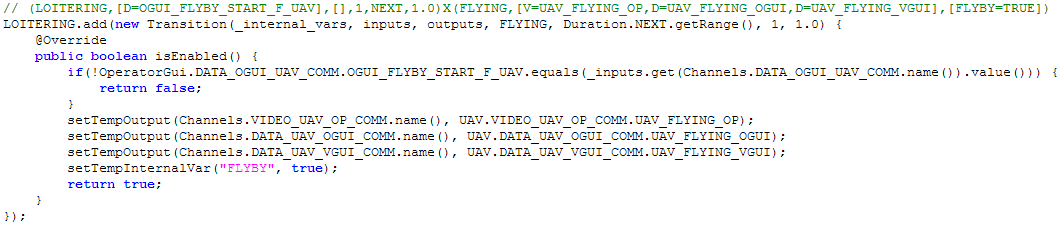
\includegraphics[width=\textwidth]{java_transition.png}
	\label{subfig:subtop}
}
\subfigure[XML Transition]{
	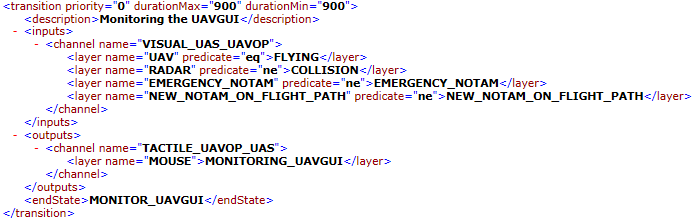
\includegraphics[width=\textwidth]{xml_transition.png}
	\label{subfig:subbot}
}
\caption{Transition Readability Comparison}
\label{fig:read_transition}
\end{center}
\end{figure}

By contrast the Enhanced Operator Function Model (EOFM), an XML based modeling language, can be visualized as a tree-like graph due to the way it is structured~\cite{bass2011toward}.  This visualization allows the modeler to see the hierarchical ordering of actions belonging to a task.  Unfortunately the use of XML to format the model did not provide a similar visualization within the Model Abstraction Framework.  In future work it may be valuable to examine a different XML structure that does allow improved visualization of the model.

\subsection{Modeling Approach and Common Errors}

In chapter~\ref{ch:xmlparser} we addressed some of the challenges of modeling within the Model Abstraction Framework.  In an effort to further reduce the time to model we developed the following modeling approach.  We first defined each Actor in the system and gave them a starting state.  From here we broke the work into task sequences.  Each task sequence represents the path or flow of data through the system, initiating from an external event.  For example our model begins with a \textit{start mission} event that is received by the UAV Operator.  We then implement transitions in sequence until no new transitions are needed.  Each time a new transition is added to the model we run the model to check that the XML is correct and to verify that the new transition is reached.  The full model can be obtained online.  See appendix~\ref{code}.

While this approach was effective it was not a trivial task.  By design the transition sequence moves between Actors requiring the modeler to constantly jump around in the model XML.  Transition sequences will often fork when the action of one Actor causes multiple Actors to respond.  This often results in truncated branches within the model that get forgotten.  In future work it may be necessary to use JPF during the model design so that all paths get checked at each iteration instead of a single path.  

One reason for running the model after adding a new transition is that when the complexity causes modeling errors they typically appear in two fashions.  The first is when an Actor becomes trapped in the current state.  This is the more desirable behavior as it is easier to track down.  The second typical error is an infinite loop.  These can be much more difficult to track down.  Infinite loops are often caused by missing transitions, which are normal during model construction.  If the loop is not caused by a missing transition then more in-depth analysis is needed to find the error.  

While there are many ways to get into an infinite loop we will only mention two common examples.  They are improper transition overriding and uncleared output channels.  Transition overriding happens when you have one transition that is overridden by another before it can fire.  While transition overriding is a desirable behavior, it simulates an interruption, gaps in the transition logic can cause an Actor to continuously cycle between transitions without ever firing a transition and moving to the next state. This can be thought of as undefined behavior.  To fix this, define the behavior for each possible scenario by creating transitions for all combinations of inputs that the Actor cares about.  The simulator will prevent a transition from replacing itself making it better to error on the side of too many transitions.  

The second common error leading to an infinite loop is uncleared outputs.  Uncleared output channels cause an Actor to believe that new input has been received even though it has not, sending the Actor into an infinite cycle.  It is often best practice to clear an Actors outputs once those outputs are no longer being sent across the channel.  This will prevent the target from reading invalid outputs.  If the output values represent a continuous communication that should not be cleared, such as displaying live state information on a GUI, then another approach is to use Actor memory to track changes in input.

While the use of XML to create the model was much more efficient we still feel that a more effective approach to modeling is needed to help standardize the modeling format and prevent common errors.  Whether this approach is a different XML structure, an entirely new format, or a GUI interface that helps visualize the data flow and transition sequences we leave to future work.

\section{Model Results}

We were very impressed with the results generated with this new case study. See Figures~\ref{fig:uavop_baseline}-\ref{fig:uavop_conflict}.  We created three scenarios by adding small variations to the model, a task that was greatly simplified by the use of XML once the initial model was complete.  The first scenario involved an uneventful flight.  The second scenario involves the UAV Operator manually avoiding an emergency NOTAM.  The third scenario involves the UAV automatically avoiding an emergency NOTAM.  The second and third scenarios also involve a possible UAV collision and the ATC adding a NOTAM onto the UAV flight path.  Additionally we added a high workload scenario that involves the UAV Operator being interrupted by another person while deconflicting the UAV.  

For each scenario we have four charts depicting the UAV Operator workload and four charts depicting the ATC workload; we currently ignore the workload for non-human Actors.  The first three charts represent the resource input, resource output, and decision workload.  The last chart shows the combined total workload next to the adapted Wickens' model.  For each chart the y axis represents the workload value while the x axis represents Actor state for the given delta time.  What this means is that the x axis cannot be seen as a normal timeline since each time step represents an arbitrary amount of time.  Instead this should be viewed as a progressive change in Actor workload for each time step where a transition was fired.

\subsection{Inter Actor Comparison}

When comparing the UAV Operator and ATC baseline workload, shown in Figures \ref{fig:uavop_baseline} and \ref{fig:atc_baseline}, the relationship between the UAV Operator and the ATC becomes very clear.  For this scenario the UAV Operator creates a flight plan for the mission.  When the UAV Operator finishes the flight plan it is sent to the FAA Server where it is flagged to be approved by the ATC.  The ATC then performs the approval and returns back to normal operations.  The UAV Operator receives the approval and begins normal mission operations that increase the workload.  This is reflected beautifully in the Actor workload.  The UAV Operator workload spikes during flight plan creation then flat lines while waiting for a response.  Once the UAV Operator receives the response their workload spikes again as they perform the mission.  The ATC workload is just the opposite, spiking while approving the flight plan and returning to normal afterwards.  The comparison of the other scenarios show the same correlations.  

\begin{figure}[p]
\begin{center}
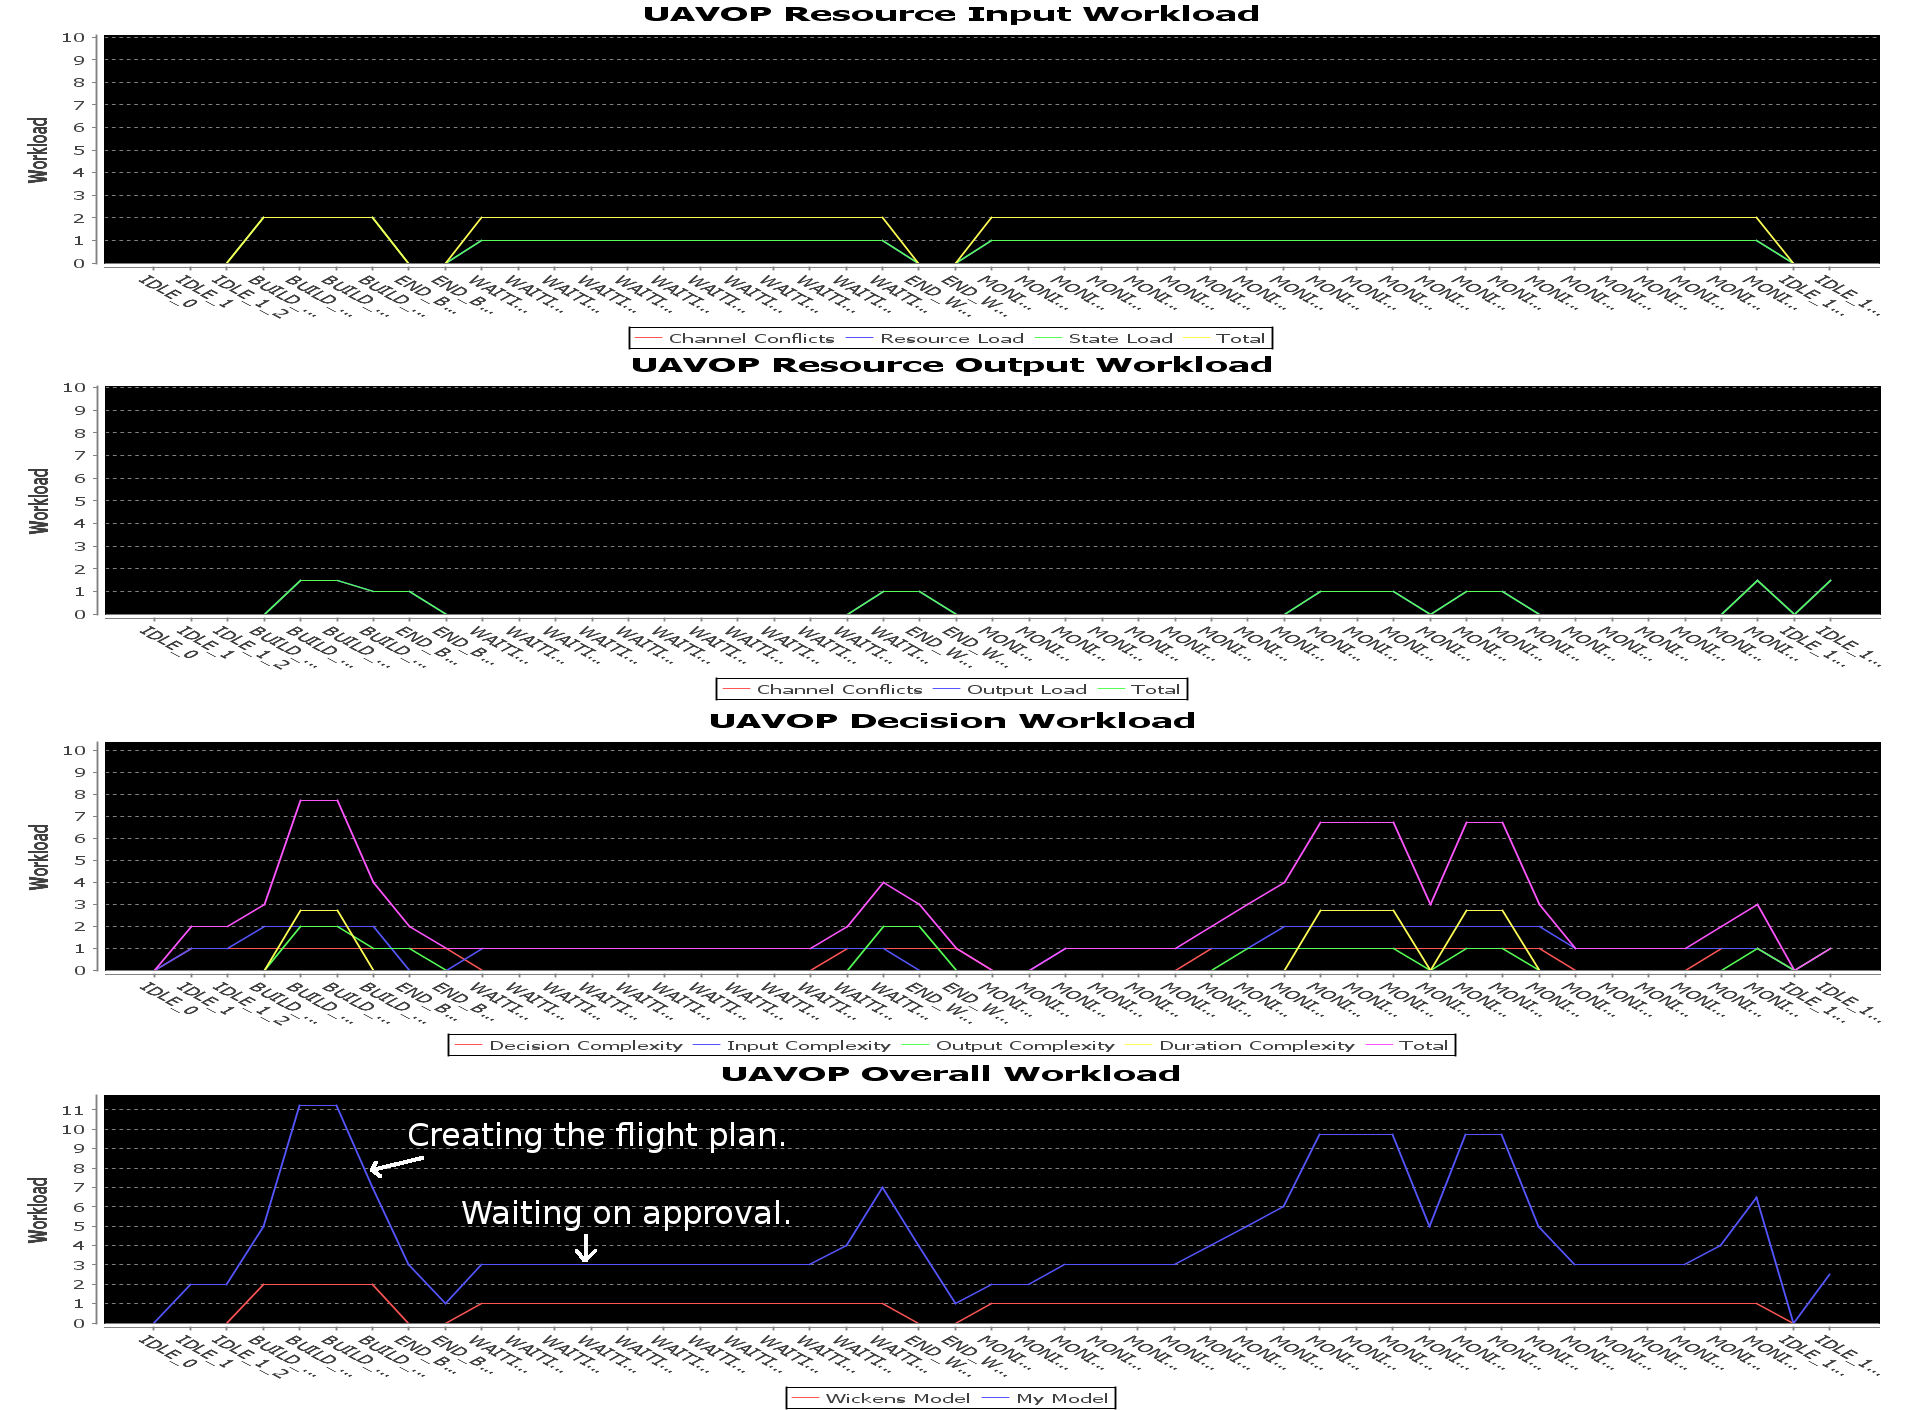
\includegraphics[width=\textwidth,height=\textheight]{UAS_in_NAS_no_events_UAVOP.png}
\vspace{-25pt}
\caption{UAV Operator: Baseline}
\label{fig:uavop_baseline}
\end{center}
\end{figure}

\begin{figure}[p]
\begin{center}
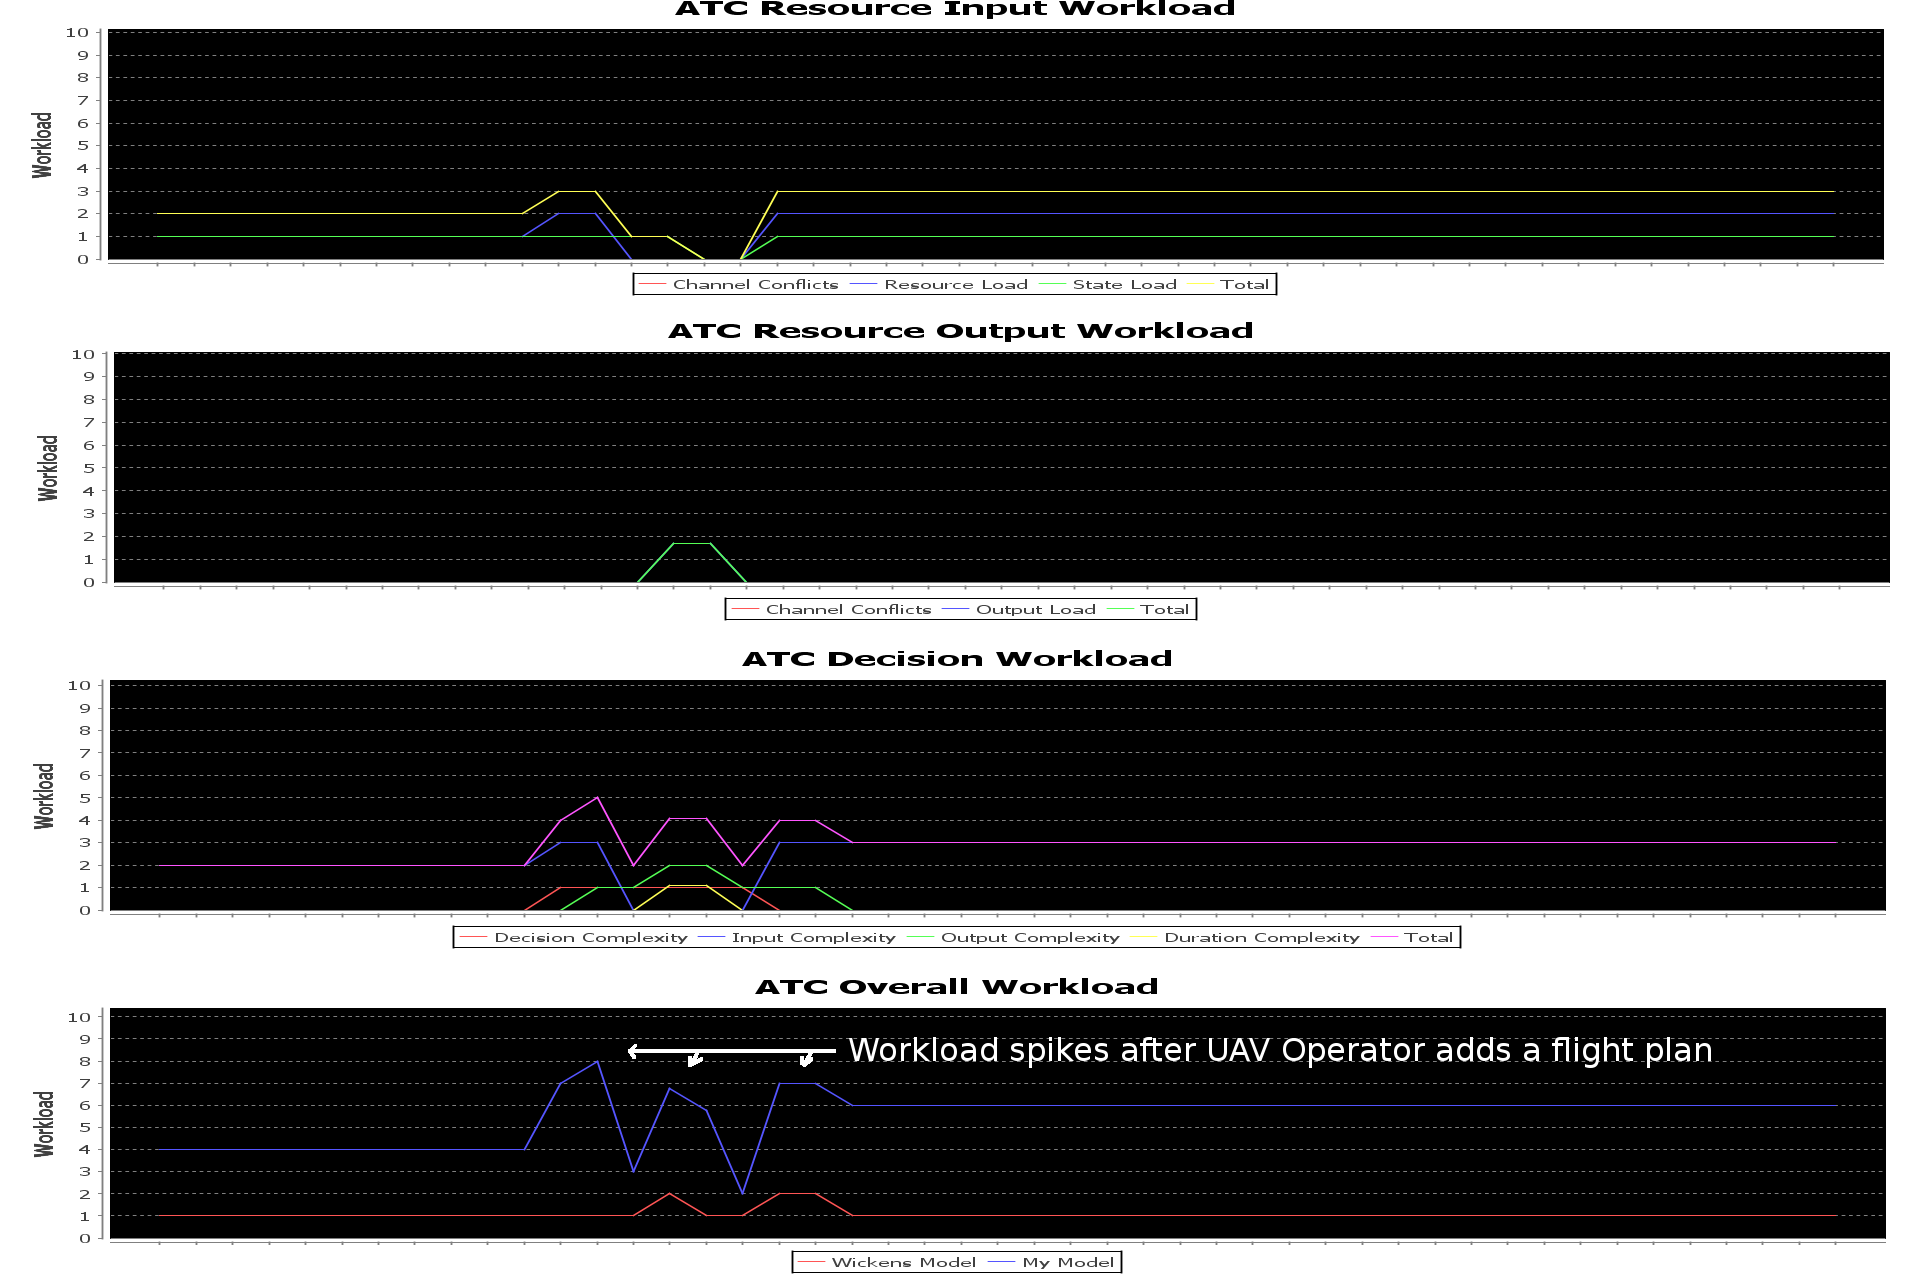
\includegraphics[width=\textwidth,height=\textheight]{UAS_in_NAS_no_events_ATC.png}
\vspace{-25pt}
\caption{ATC: Baseline}
\label{fig:atc_baseline}
\end{center}
\end{figure}

We also see the effects of the UAV Operator and ATC relationship in the \textit{manual avoid} scenario, shown in Figures~\ref{fig:uavop_manual} and \ref{fig:atc_manual}, when the delayed action of the UAV Operator causes the ATC to remain in the \textit{avoid conflict} state for an abnormally long period of time.  By looking at the Actor state we see that the UAV Operator was already in the process of deconflicting the UAV and was not able to immediately respond to the ATC emergency NOTAM.  The \textit{auto avoid} scenario, shown in Figures~\ref{fig:uavop_auto} and \ref{fig:atc_auto}, shows an improvement in this regard as the UAV automatically avoids the emergency NOTAM while the UAV Operator is busy.  This example demonstrates how the workload modeling allows us to detect problems using the model and then analyze fixes to those problems.

\begin{figure}[p]
\begin{center}
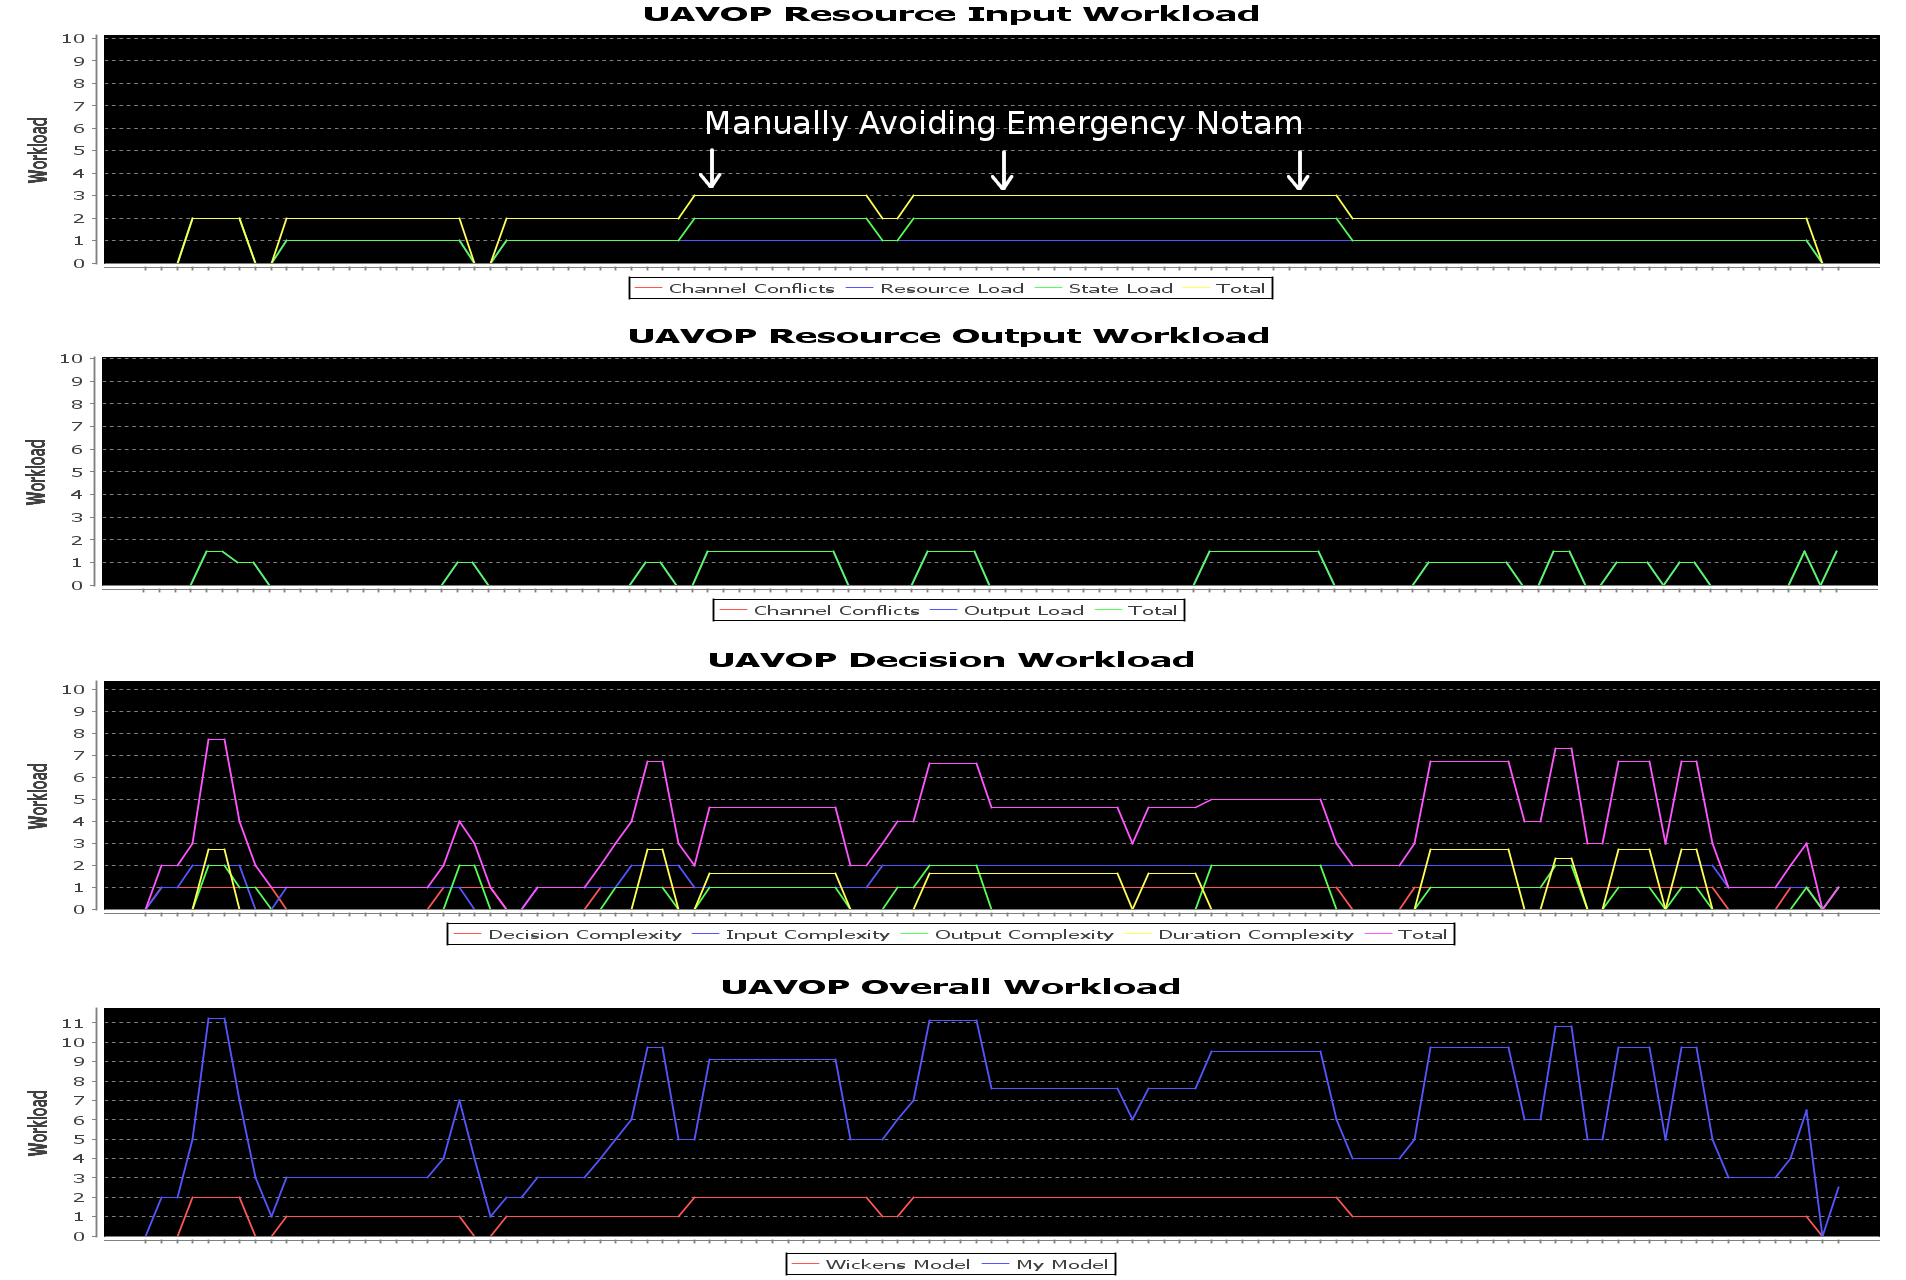
\includegraphics[width=\textwidth,height=\textheight]{UAS_in_NAS_manual_emergency_notam_UAVOP.png}
\vspace{-25pt}
\caption{UAV Operator: Manually Avoided Emergency NOTAM}
\label{fig:uavop_manual}
\end{center}
\end{figure}

\begin{figure}[p]
\begin{center}
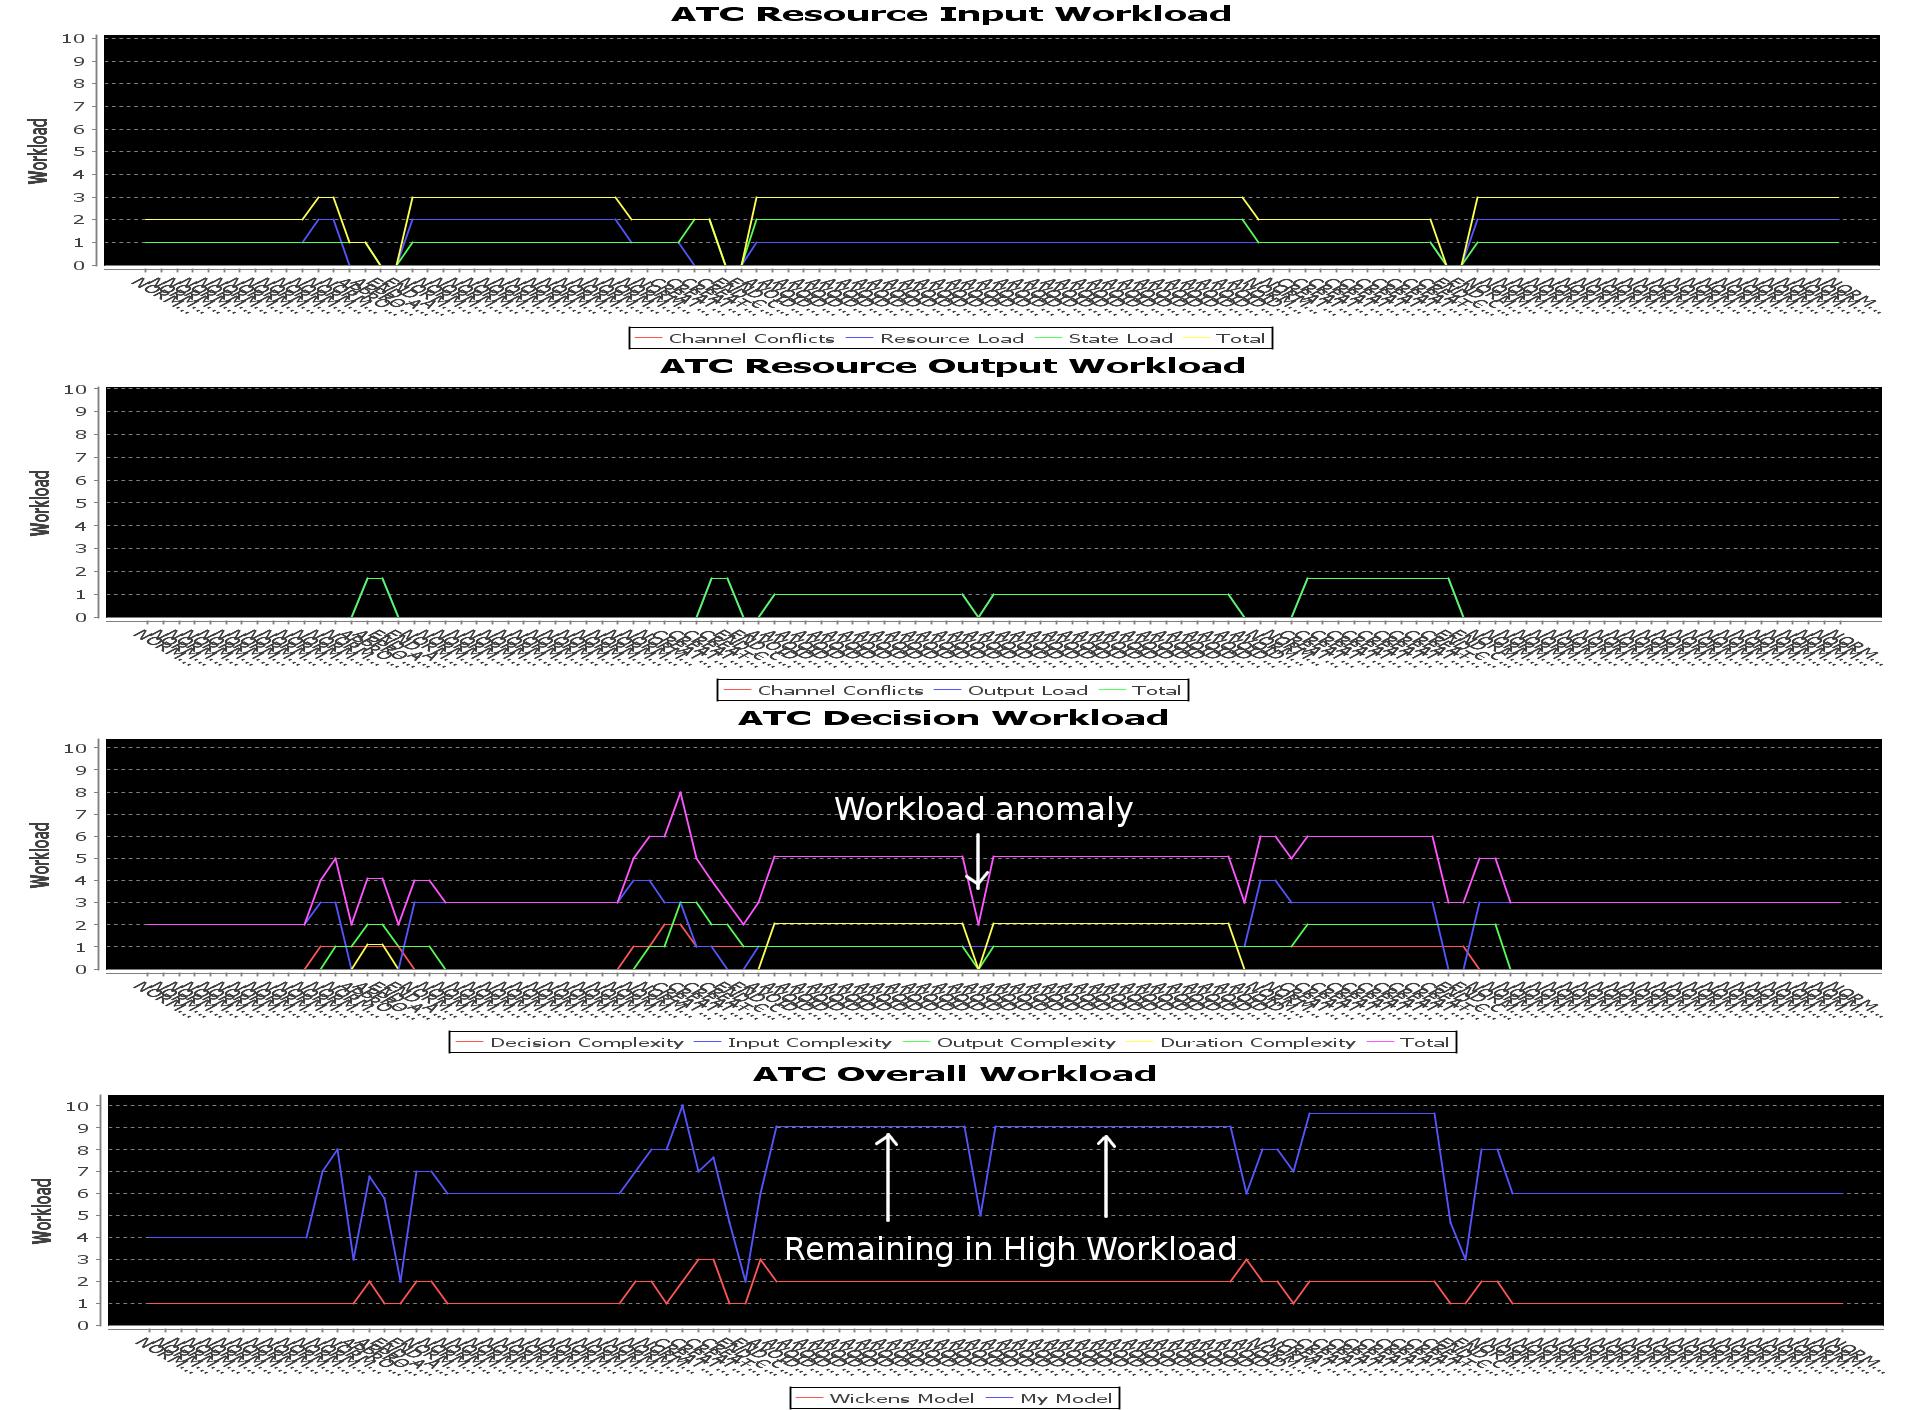
\includegraphics[width=\textwidth,height=\textheight]{UAS_in_NAS_manual_emergency_notam_ATC.png}
\vspace{-25pt}
\caption{ATC: Manually Avoided Emergency NOTAM}
\label{fig:atc_manual}
\end{center}
\end{figure}

\subsection{Intra Actor Comparison}

At first glance the UAV Operator workload between the \textit{manual avoid} scenario, Figure~\ref{fig:uavop_manual}, and the \textit{auto avoid} scenario, Figure~\ref{fig:uavop_auto}, appear almost identical.  This is good as these scenarios are nearly identical.  Upon closer examination we see that when the UAV Operator has to manually avoid the emergency NOTAM there is a prolonged increase in resource input workload, an extra spike of resource output workload, and a noticeable spike in decision workload once the UAV Operator begins the process of avoiding the NOTAM.  This results in a significant workload spike compared to the more stable workload seen in the \textit{auto avoid} scenario.  Another less noticeable difference is that the manual emergency NOTAM avoidance takes longer to complete than the auto avoid feature, something that is critical in these types of situations.

\begin{figure}[p]
\begin{center}
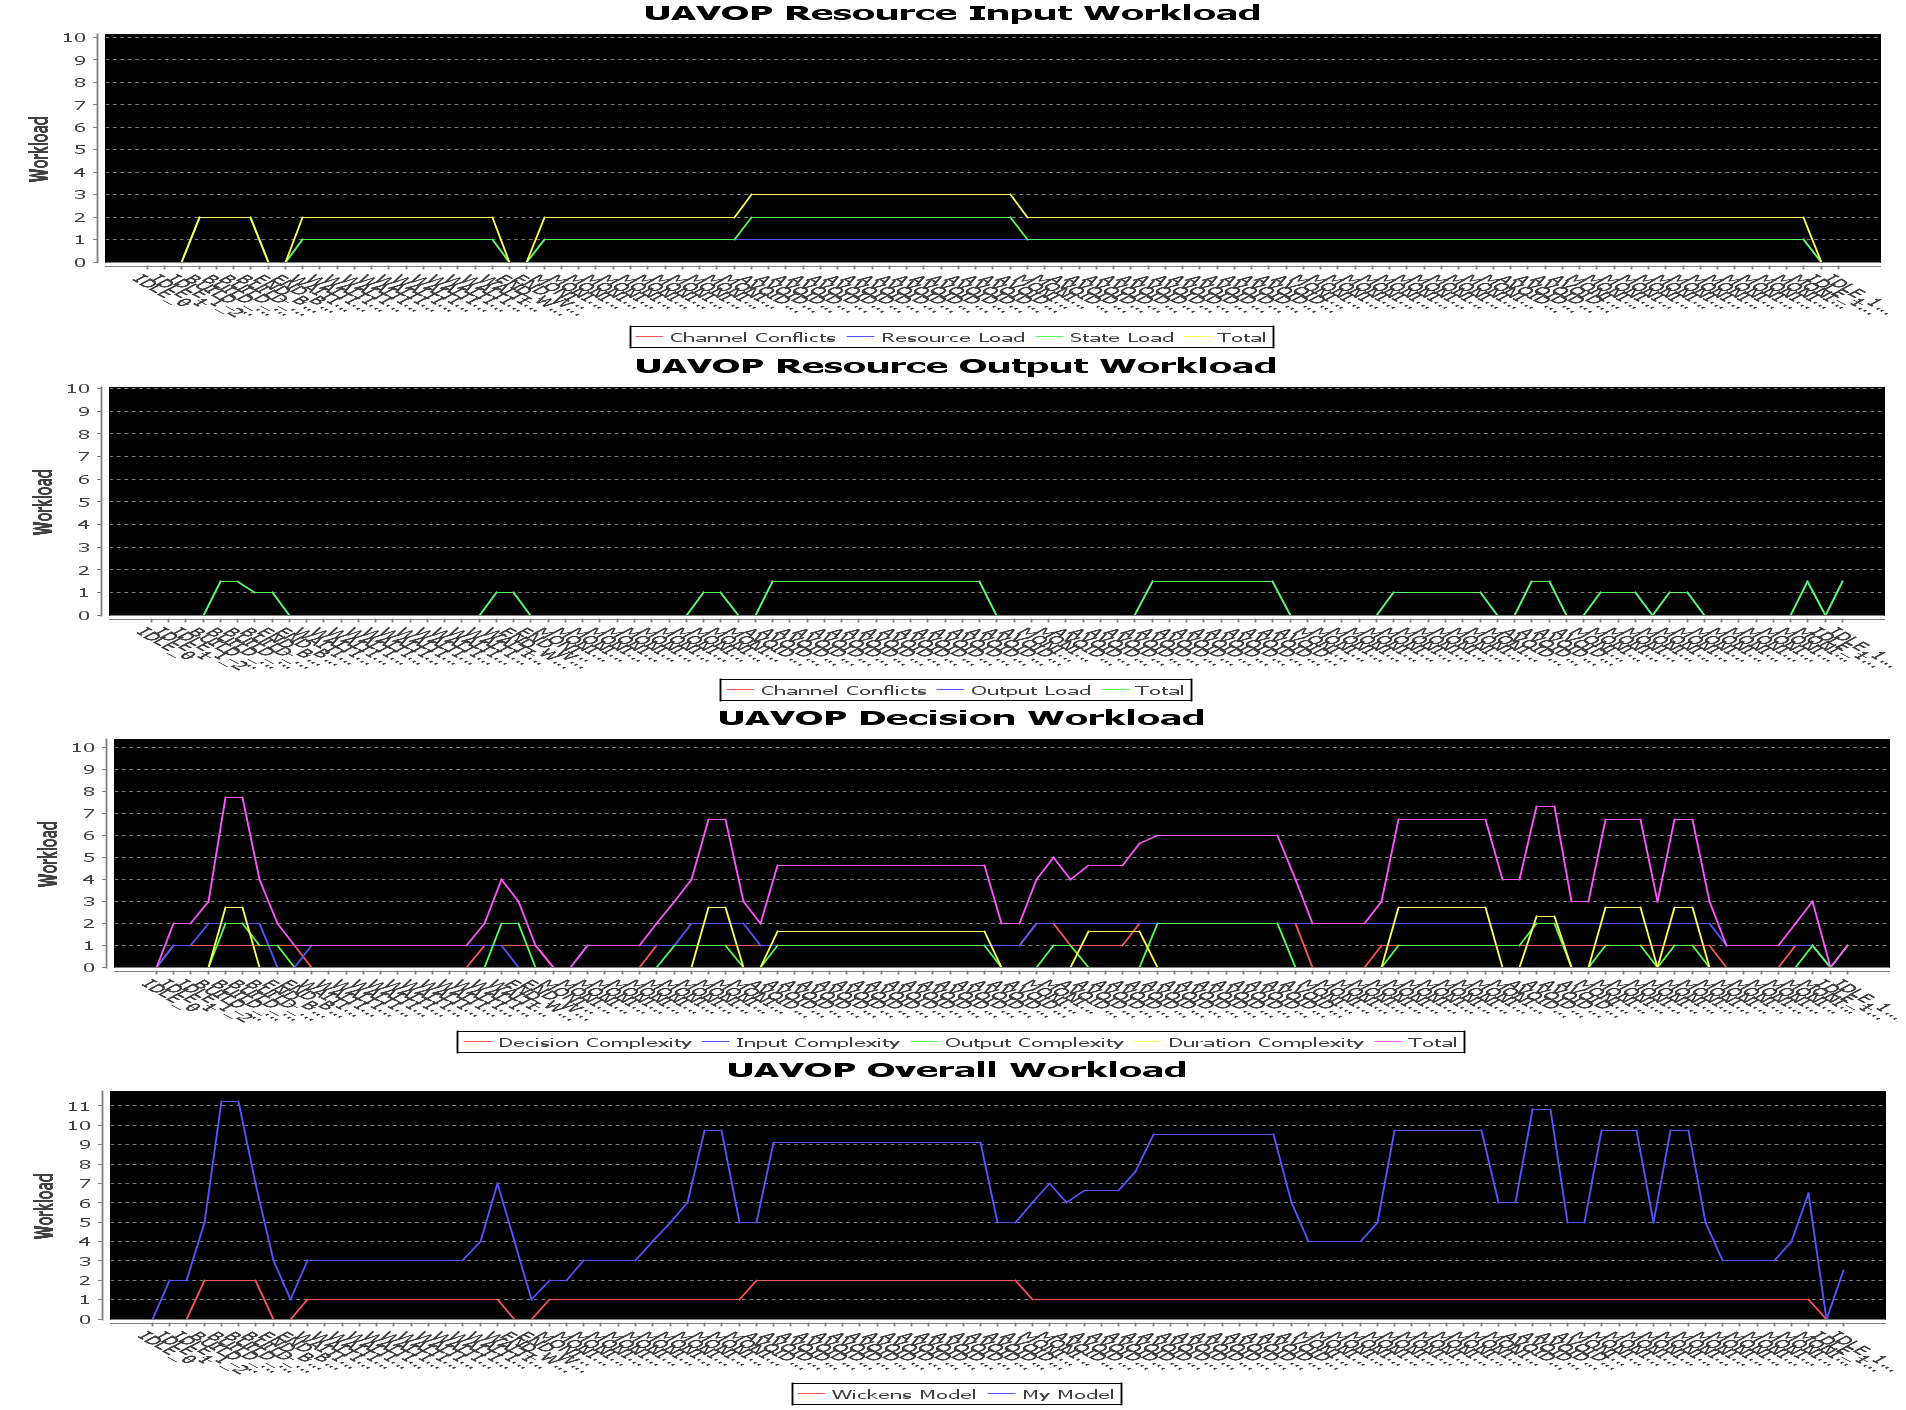
\includegraphics[width=\textwidth,height=\textheight]{UAS_in_NAS_auto_emergency_notam_UAVOP.png}
\vspace{-25pt}
\caption{UAV Operator: Auto Avoid Emergency NOTAM}
\label{fig:uavop_auto}
\end{center}
\end{figure}

\begin{figure}[p]
\begin{center}
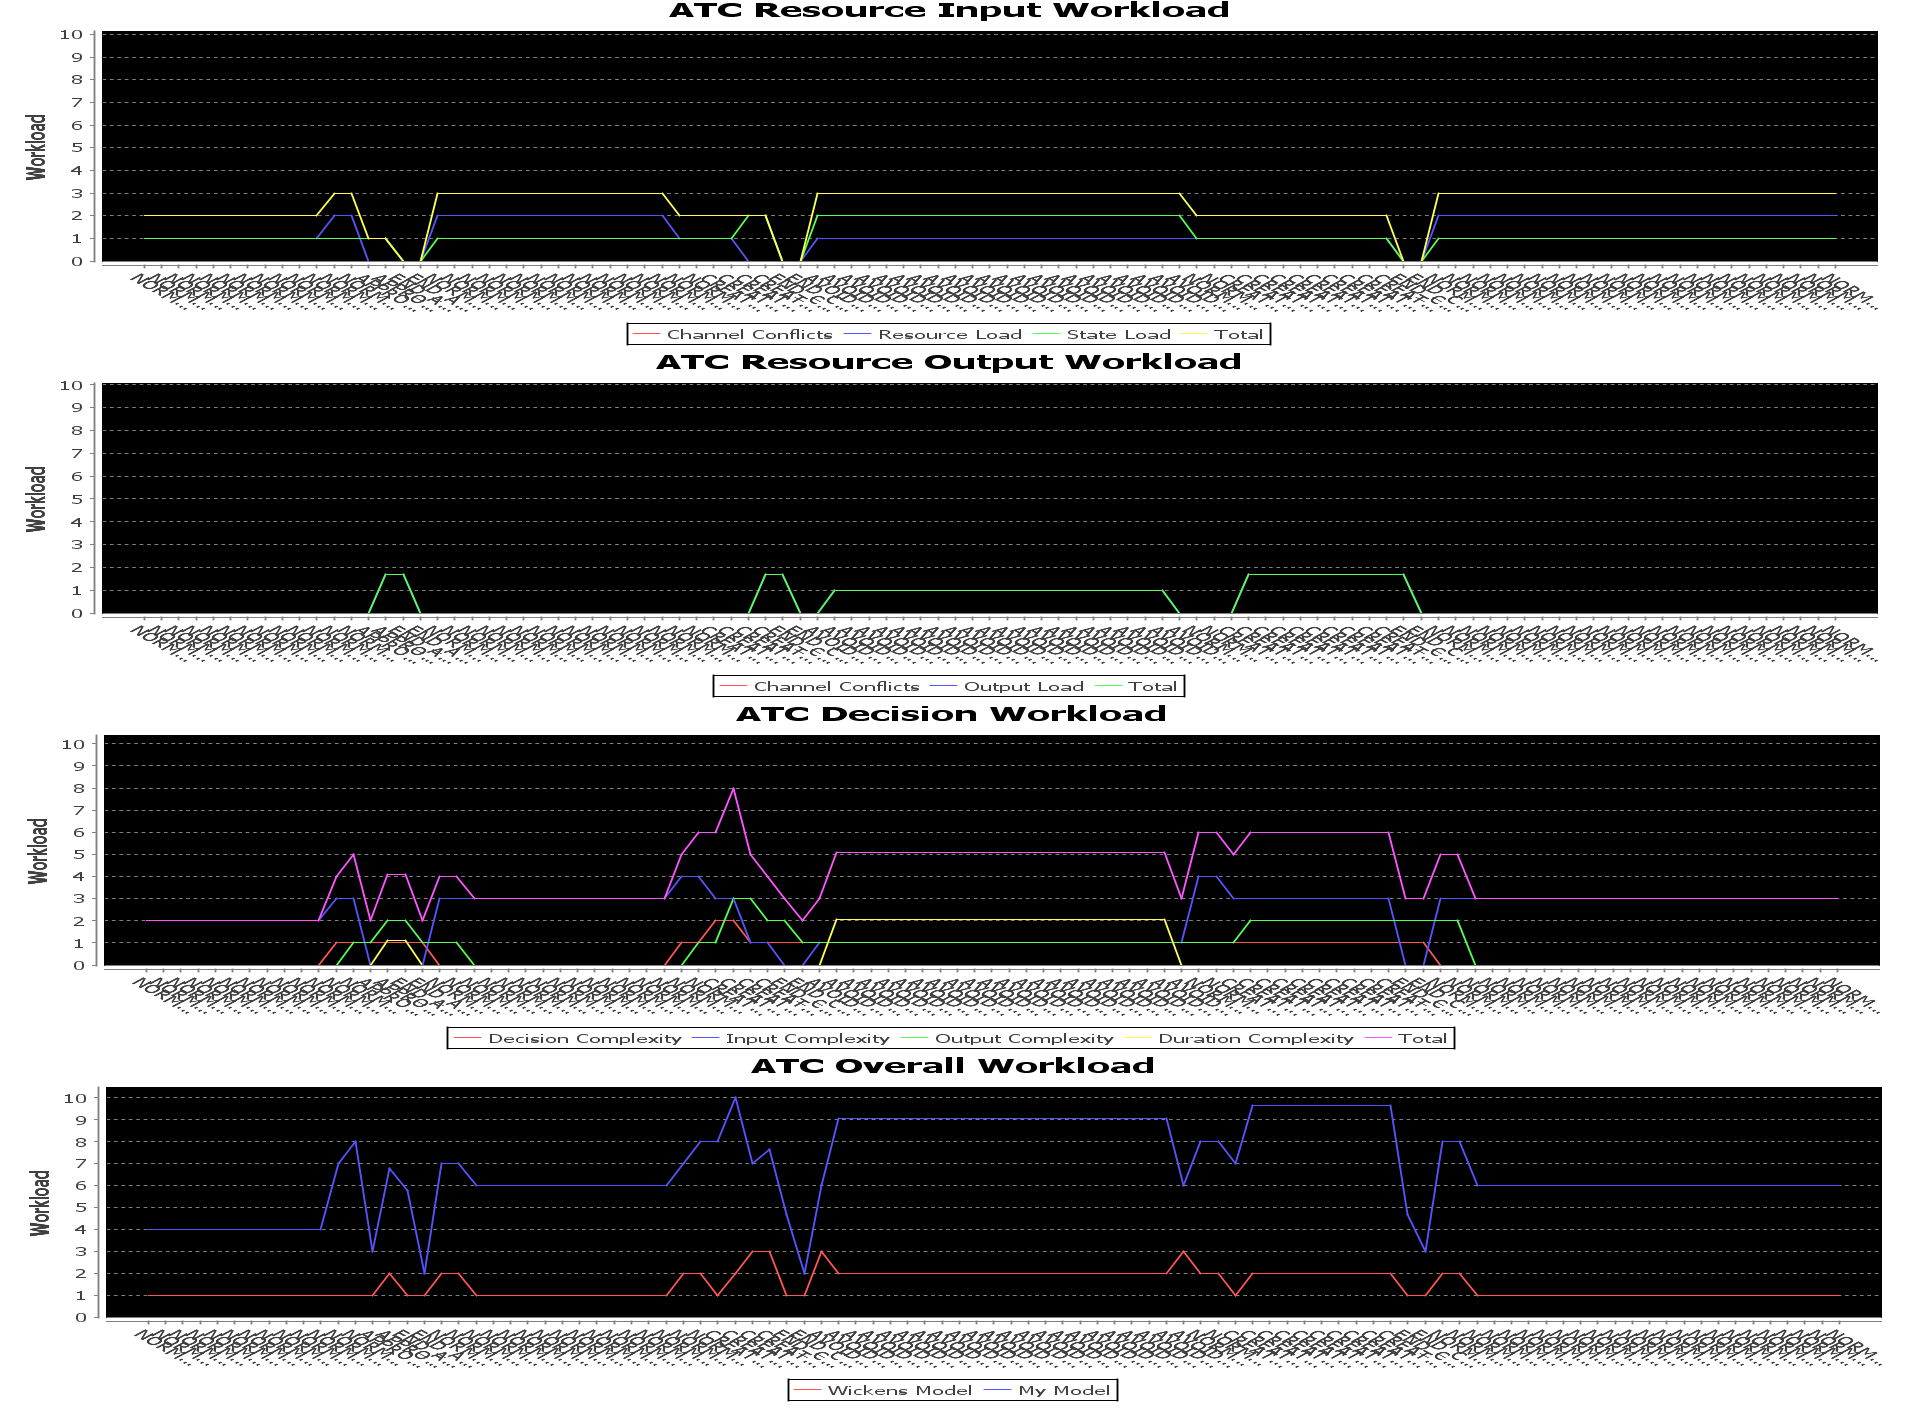
\includegraphics[width=\textwidth,height=\textheight]{UAS_in_NAS_auto_emergency_notam_ATC.png}
\vspace{-25pt}
\caption{ATC: Auto Avoid Emergency NOTAM}
\label{fig:atc_auto}
\end{center}
\end{figure}

To make this simple model a little more interesting we decided to add an interruption to the \textit{auto avoid} scenario.  See Figure \ref{fig:uavop_conflict}.  When the UAV Operator begins the first deconfliction procedure he or she is interrupted by another person, a dummy Actor added to the model just for this interruption.  Instead of ignoring this interruption the UAV Operator attempts to communicate with this person while still performing the deconfliction procedure.  This results in a visual channel conflict as the UAV Operator is watching both the UAS GUI and the person that caused the interruption.  In addition to this the UAV Operator is now in a high load/multi tasking state.  The result is a workload value of 20, almost double the next highest workload value seen in the simulation.

\begin{figure}[p]
\begin{center}
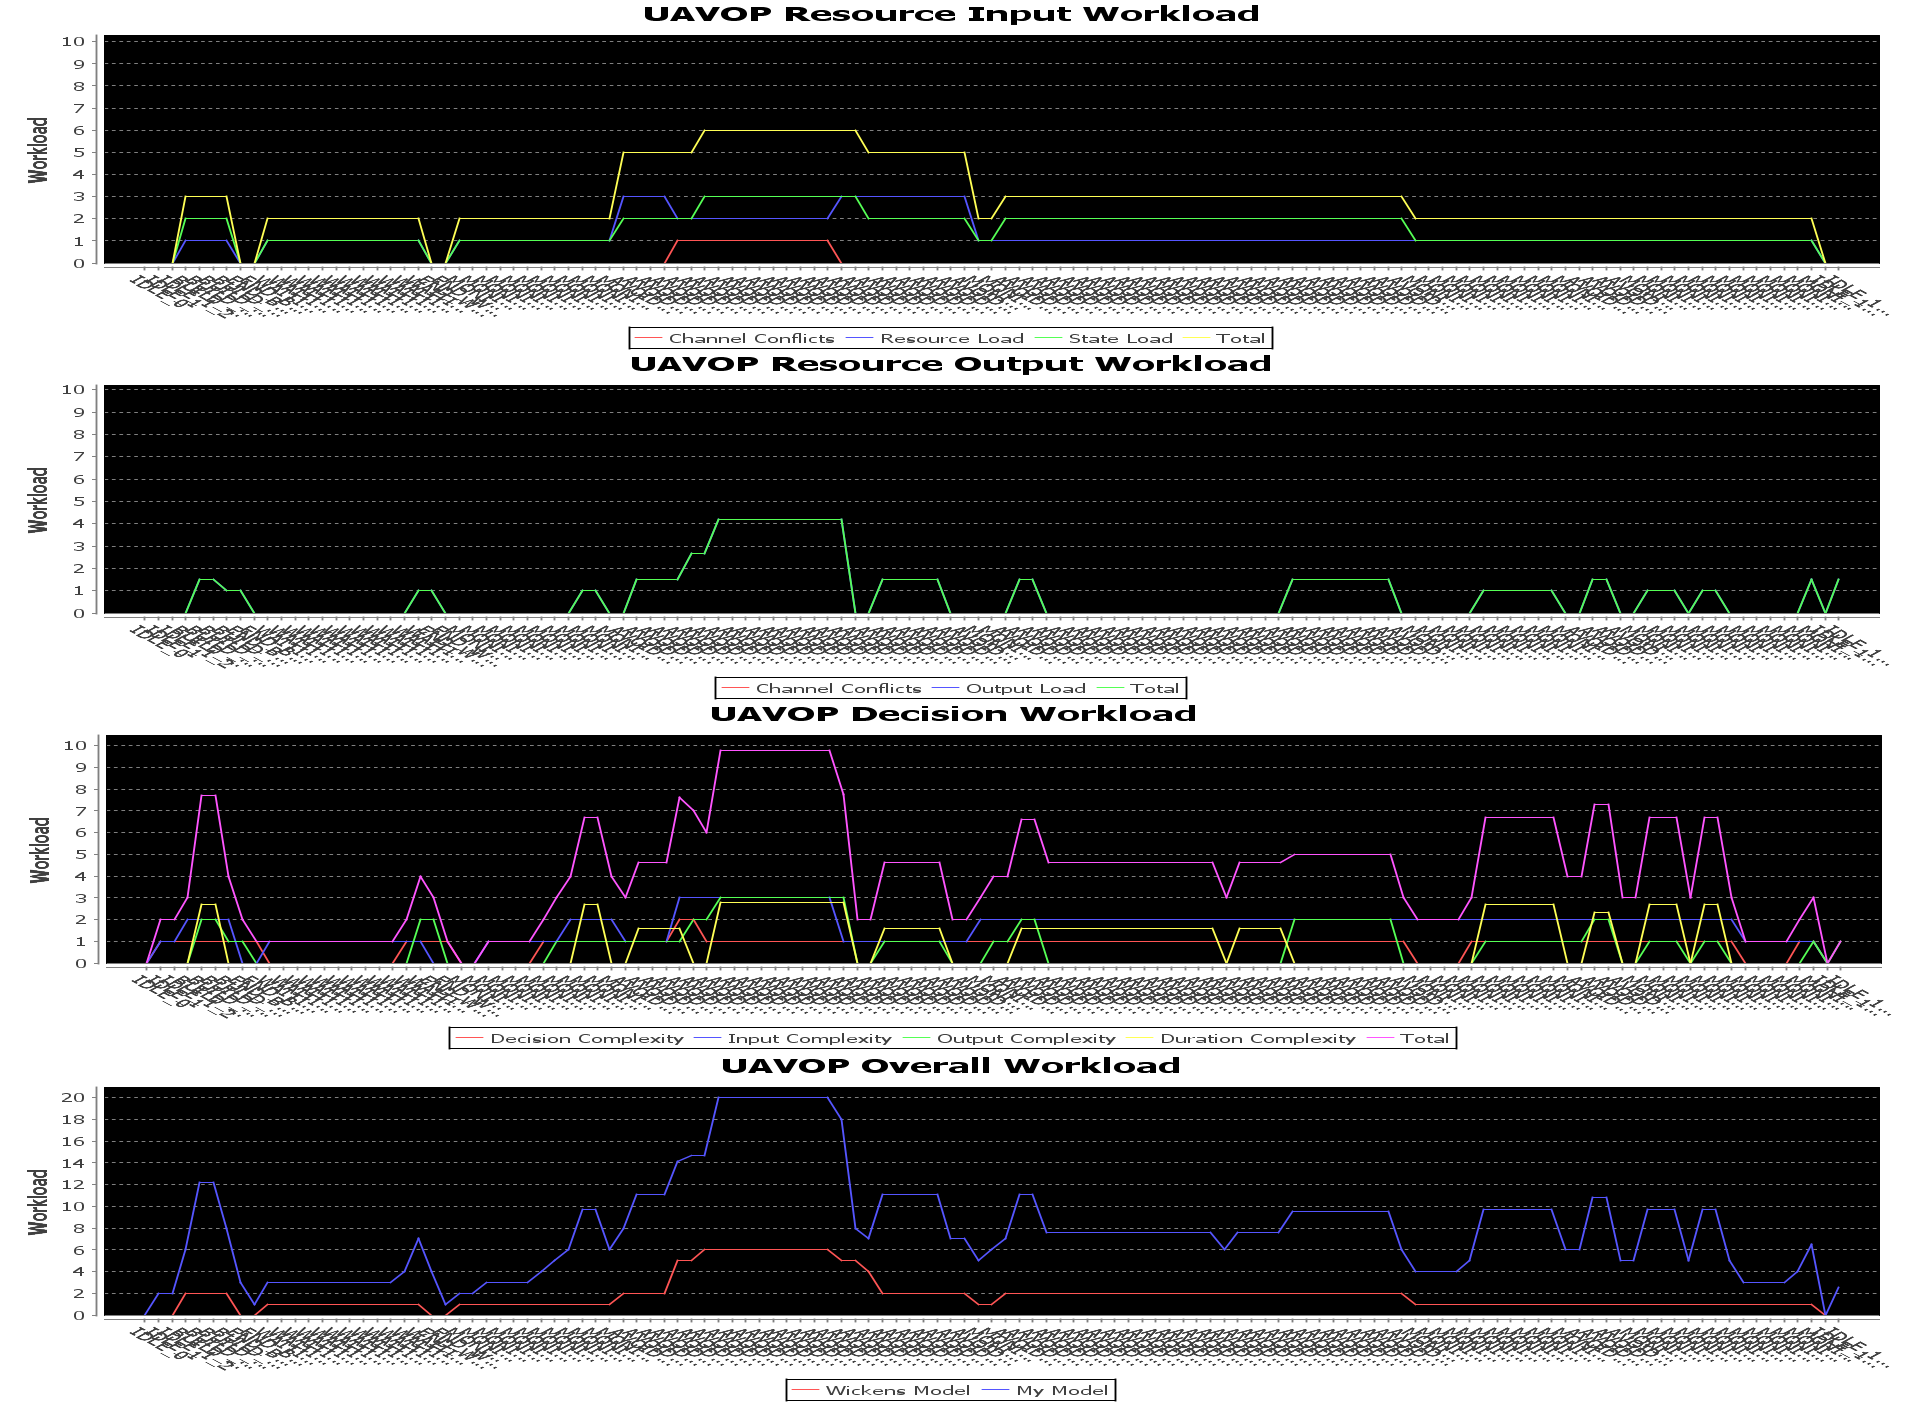
\includegraphics[width=\textwidth,height=\textheight]{UAS_in_NAS_channel_conflict_UAVOP.png}
\vspace{-25pt}
\caption{UAVOP: Auto Avoid Emergency NOTAM w/ Interruption}
\label{fig:uavop_conflict}
\end{center}
\end{figure}

While we are mostly pleased with the workload results there are a few anomalies in the results that are misleading.  The most commonly occurring anomaly is a drastic decrease in workload followed immediately be an equally drastic increase in workload, see figure~\ref{fig:atc_manual}.  This tends to happen when an Actor is transitioning into the same state it just left.  The spike happens because we are collecting metrics twice for each step in the delta clock; once right before the active transitions are fired and once after they are fired.  In future work we may collect specific metrics once per delta clock step to prevent these anomalies.

\subsection{Workload Analysis}

To view the metric data more clearly we split the data into four different charts that represent the \textit{resource input workload}, \textit{resource output workload}, \textit{decision workload}, and \textit{overall workload}.  In the \textit{resource input workload} chart we get an idea of how many channels, layers, and memory objects the Actor is observing.  By comparing this with the \textit{resource output workload} we can see when the inputs occasioned a response from the Actor.  For the most part these charts are well behaved and follow the workload patterns that we know about.

On the other hand the \textit{decision workload} typically jumps all over the place.  While we believe the increase in \textit{decision workload} does in fact increase \textit{overall workload}, we are unsure how to weight this value in comparison with the \textit{resource workload} and \textit{temporal workload}.  This is something that needs to be verified through sensitivity and user studies in future work.

The last analysis we would like to make is the comparison of our workload metric to that of the adapted Wickens' model from chapter~\ref{ch:metrics}.  The general flow of the two metrics is very similar, as is expected since everything in the Wickens' model also exists in our workload metric.  What is more interesting is where the two metrics differ.  Our workload metric is comprised of 9 different values each of which can range from zero to two or more.  This adds a fair amount of detail into the workload measurement.  An example of this can be seen in the \textit{auto avoid} scenario shown in Figure~\ref{fig:uavop_auto}.  After avoiding the emergency NOTAM the UAV Operator continues to monitor the UAS GUI eventually avoiding another potential conflict.  The adapted Wickens' model shows a flat line during this portion of the scenario while our metric shows a heart beat that correlates with the UAV Operator actions.  

